\documentclass[tikz, border=6pt]{standalone}
\IfFileExists{lmodern.sty}{\usepackage[T1]{fontenc}\usepackage{lmodern}}{}
\usepackage{amsmath,amssymb,bm}
\usepackage[scaled=0.95]{helvet}
\usetikzlibrary{arrows.meta, decorations.pathreplacing}
\definecolor{Blue}{HTML}{3A76D8}
\definecolor{Teal}{HTML}{16A394}
\definecolor{Ink}{HTML}{1F2937}
\tikzset{
  dot/.style={circle, fill, inner sep=0pt, minimum size=4.5pt},
  block/.style={/utils/exec={\colorlet{pytikzarg}{#1}}, draw=pytikzarg!78!black, fill=pytikzarg!14, rounded corners=3pt, align=center, inner sep=5pt, minimum height=8mm, minimum width=20mm},
  block/.default=Blue,
  op/.style={circle, draw, fill=white, inner sep=0pt, minimum size=5mm, font=\normalsize},
}
\begin{document}
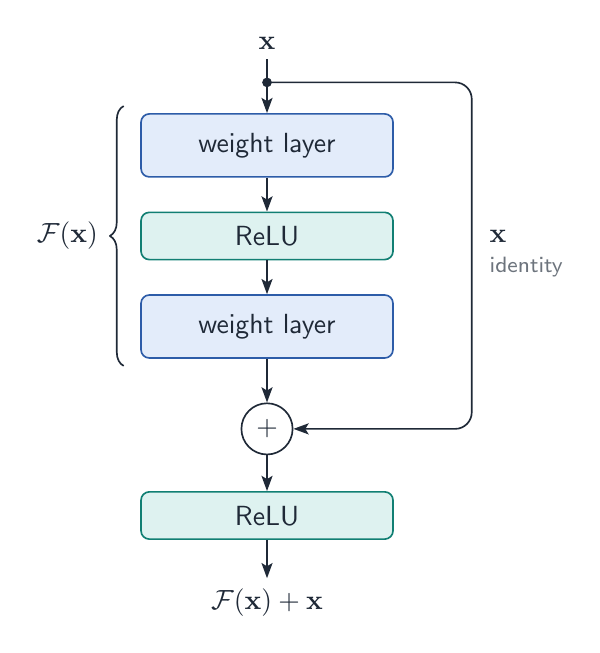
\begin{tikzpicture}[color=Ink, execute at begin picture={\sffamily}, line width=0.6pt, >={Stealth[length=5.5pt, width=4pt, inset=1.2pt]}, line join=round]
  \node (n1) at (0,0) {$\mathbf{x}$};
  \node[block=Blue, minimum width=3.2cm] (n2) at (0,-1.3) {weight layer};
  \node[block=Teal, minimum width=3.2cm, minimum height=0.6cm] (n3) at (0,-2.45) {ReLU};
  \node[block=Blue, minimum width=3.2cm] (n4) at (0,-3.6) {weight layer};
  \node[op, minimum size=0.65cm] (n5) at (0,-4.9) {$+$};
  \node[block=Teal, minimum width=3.2cm, minimum height=0.6cm] (n6) at (0,-6) {ReLU};
  \node (n7) at (0,-7.1) {$\mathcal{F}(\mathbf{x}) + \mathbf{x}$};
  \draw[->] (n1) -- (n2);
  \draw[->] (n2) -- (n3);
  \draw[->] (n3) -- (n4);
  \draw[->] (n4) -- (n5);
  \draw[->] (n5) -- (n6);
  \draw[->] (n6) -- (n7);
  \node[dot, minimum size=3.5pt] at (0,-0.5) {};
  \draw[->, rounded corners=6pt] (0,-0.5) -- (2.6,-0.5) -- (2.6,0 |- n5) -- (n5.east);
  \node[anchor=west, xshift=0.1cm] at (2.6,-2.45) {$\mathbf{x}$};
  \node[anchor=west, xshift=0.1cm, font=\footnotesize, text=Ink!65] at (2.6,-2.85) {identity};
  \draw[decorate, decoration={brace, amplitude=5pt, raise=2pt}] (-1.75,-4.1) -- (-1.75,-0.8)
      node[midway, auto, outer sep=8pt] {$\mathcal{F}(\mathbf{x})$};
\end{tikzpicture}
\end{document}
